\documentclass{beamer}
\usepackage{beamerthemesplit}
\usetheme{Madrid}
\usecolortheme{seagull}
\usepackage{makeidx}
\usepackage{seamless-beamer}
\usepackage{listings}
\lstdefinelanguage{chapel}
  {
    morekeywords={
      align, atomic,
      begin, bool, break, by,
      class, cobegin, coforall, complex, config, const, continue,
      delete, dmapped, do, domain,
      else, enum, extern, export,
      false, for, forall,
      if, imag, in, index, inline, inout, int, iter,
      label, lambda, let, local, locale,
      module,
      new, nil, noinit,
      on, opaque, otherwise, out,
      param, proc,
      range, real, record, reduce, ref, return,
      scan, select, serial, single, sparse, string, subdomain, sync,
      then, true, type,
      uint, union, use,
      var,
      when, where, while, with,
      yield,
      zip
    },
    sensitive=false,
    mathescape=true,
    morecomment=[l]{//},
    morecomment=[s]{/*}{*/},
    morestring=[b]",
}

\lstset{
    basicstyle=\footnotesize\ttfamily,
    keywordstyle=\bfseries,
    commentstyle=\em,
    showstringspaces=false,
    flexiblecolumns=false,
    numbers=left,
    numbersep=5pt,
    numberstyle=\tiny,
    numberblanklines=false,
    stepnumber=0,
    escapeinside={(*}{*)},
    language=chapel,
  }

%\newcommand{\chpl}[1]{\lstinline[language=chapel,basicstyle=\ttfamily,keywordstyle=\bfseries]!#1!}
\newcommand{\chpl}[1]{\lstinline[language=chapel,basicstyle=\small\ttfamily,keywordstyle=]!#1!}
\newcommand{\varname}[1]{\emph{#1}}
\newcommand{\typename}[1]{\emph{#1}}
\newcommand{\fnname}[1]{\chpl{#1}}

\lstnewenvironment{chapel}{\lstset{language=chapel,xleftmargin=2pc,stepnumber=0}}{}
\lstnewenvironment{invisible}{\lstset{language=chapel,xleftmargin=2pc,stepnumber=0,keywordstyle=\bfseries\color{white},basicstyle=\small\ttfamily\color{white}}}{}
\lstnewenvironment{chapel0}{\lstset{language=chapel,stepnumber=0}}{}

\lstnewenvironment{numberedchapel}{\lstset{language=chapel,xleftmargin=15pt,stepnumber=1}}{}

\lstnewenvironment{chapelcode}{\lstset{language=chapel,stepnumber=1}}{}

% Uses the same listing style as the {chapel} environment, but keyword
% formatting is turned off.  The argument is ignored in LaTeX
% but used to name the .good file during test extraction.
% The argument must be supplied but may be empty.
% If empty it defaults to null, which signals the test extractor to 
% autogenerate the .good file name as ``<test_name>.good''.
\lstnewenvironment{chapelprintoutput}[1]
  {\lstset{language=chapel,xleftmargin=2pc,stepnumber=0,keywordstyle=}}{}

\lstnewenvironment{commandline}{\lstset{keywordstyle=,xleftmargin=2pc}}{}

\lstnewenvironment{protohead}{\lstset{language=chapel,xleftmargin=0pc,belowskip=-10pt,stepnumber=0}}{}

\newenvironment{protobody}{\begin{description}\item[\quad\quad] }{\end{description}}

\renewcommand{\ttdefault}{pcr}
\mode<presentation>
\makeindex
\newenvironment{theindex}
{\let\item\par
  %definitions for subitem etc
}{}
\newcommand\indexspace{}

% some custom latex convenience commands
\usepackage{xspace}
\newcommand*{\eg}{\emph{e.g.}\@\xspace}
\newcommand*{\ie}{\emph{i.e.}\@\xspace}
\newcommand*{\seamless}{\texttt{seamless}\@\xspace}
\newcommand*{\latex}{\LaTeX\@\xspace}

\makeatletter
\newcommand*{\etc}{%
  \@ifnextchar{.}%
  {etc}%
  {etc.\@\xspace}%
}
\makeatother

{ \usetheme{boxes} }
\title[\seamless Introduction]{Code Development with \texttt{seamless}: Introduction}
\author[Adamson]{Paul Adamson \\ \texttt{paul.adamson.01@gmail.com}}
\date{January 29, 2015}

%\AtBeginSection[]
%{
  %\begin{frame}
    %\frametitle{Outline}
    %\tableofcontents[currentsection]
  %\end{frame}
%}

\begin{document}
\begin{frame}
  \titlepage
\end{frame}

\begin{frame}
  \frametitle{Outline}
  \tableofcontents
\end{frame}

\section{Motivation for \texttt{seamless}}
\begin{frame}
  \frametitle{Motivation for \seamless}
  \begin{itemize}
    \item a lot of legacy code will be rewritten over the next couple of decades
    \item many incentives to producing reusable, maintainable code\cite{petre}
    \item some significant roadblocks 
      \begin{itemize}
        \item we are scientists first, programmers second (or third, fourth...)
        \item high overhead of integrating multiple software engineering tools
        \item we think $cost > benefit$
      \end{itemize}
    \item need a lightweight, easy to use system to implement good software engineering
      practices
    \item targeting small- to moderately-sized software projects
    \item not looking to develop a template for all projects---tool will be extensible \& adaptable
  \end{itemize}
\end{frame}


\section{Test-Driven Development}
\subsection{Typical Test-Driven Development (TDD) Process}
\begin{frame}
  \frametitle{Typical Test-Driven Development (TDD) Process\cite{tdd-wikipedia}}
\index{test-driven development process}
  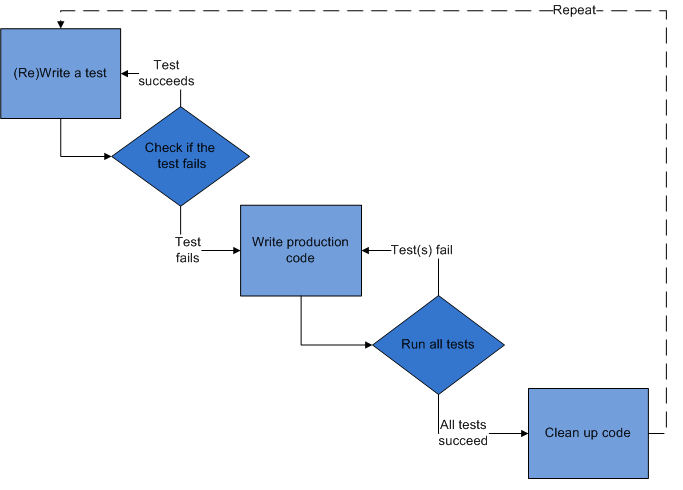
\includegraphics[scale=0.45]{fig/test-driven_development.png}
\end{frame}

\subsection{Characteristics of Test-Driven Development}
\begin{frame}
  \frametitle{Characteristics of Test-Driven Development}\index{test-driven development characteristics}
  \begin{itemize}
    \item \textit{write the test} for a feature \textit{before writing the code}
    \item aids design
      \begin{itemize}
        \item forces systematic thinking about code functionality and interfaces
        \item problem is decomposed into small, modular increments
      \end{itemize}
    \item resulting code is robust and maintainable 
      \begin{itemize}
        \item completely covered by tests
        \item accurate
        \item low coupling, minimal side effects, high cohesion
        \item well-factored, easier to modify
      \end{itemize}
    \item tests are a form of documentation
  \end{itemize}
\end{frame}

\section{Literate Programming}
\begin{frame}
  \frametitle{Literate Programming}
  \begin{itemize}
    \item reverse code/documentation weighting and development cycles
      \begin{itemize}
        \item a lot of code with scant ``comment delimited'' plain text documentation versus
        \item thorough, well-organized, and content-rich documentation with modular and efficient code
      \end{itemize}
    \item high-level language code and associated documentation come from the same set of source files
    \item mathematics and graphics included in documentation
  \end{itemize}
\end{frame}

\subsection{Literate Program Requirements}
\begin{frame}
  \frametitle{Literate Program Requirements\cite{childs}}\index{literate program requirements}
  \begin{enumerate}
    \item code and documentation in same source
    \item documentation and associated code adjacent 
    \item subdivided in a logical way
    \item logical presentation versus conforming to syntactic constraints
    \item includes open issues, rationales, \etc 
    \item description of the problem and solution
      (all the math and graphics necessary)
    \item automatic cross references, indices, and different fonts for text, keywords, 
      variable names, and literals 
    \item written in small chunks including documentation, definitions, and code
  \end{enumerate}
\end{frame}

\subsection{A Quasi-Literate Programming Example}
\begin{frame}[fragile]
  \frametitle{A Quasi-Literate Programming Example}
  We want to integrate the function $f(x) = (2 x-0.5)^3+(1.5 x-1)^2-x+1$ for $x$ in $[0.1,0.8]$
  \begin{columns}[onlytextwidth]
    \begin{column}{0.3\textwidth}
      using the right rectangle numerical integration method. This method is illustrated in 
      the figure to the right.
    \end{column}
    \begin{column}{0.1\textwidth}
    \end{column}
    \begin{column}{0.6\textwidth}
      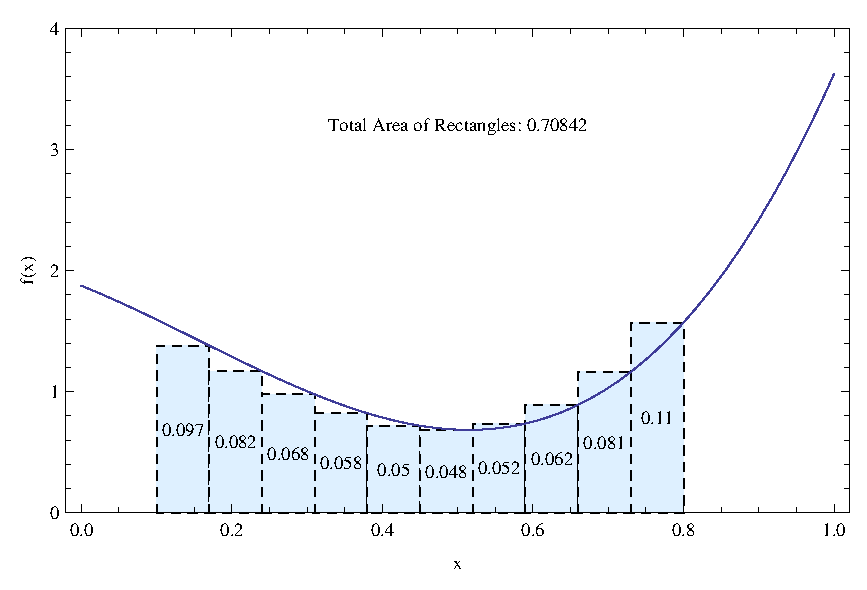
\includegraphics[scale=.45]{../../fig/rightrectangle-10.eps}
    \end{column}
  \end{columns}
  \textit{Helper (testFunctions.chpl)}. Provides the function $f(x) = (2 x-0.5)^3+(1.5 x-1)^2-x+1$.
  \begin{chapel}
proc f(x:real):real {
  return (2 * x - 0.5)**3 + (1.5 * x - 1)**2 - x + 1;
} 
  \end{chapel}
\end{frame}

\subsection{Un-\texttt{tangle} a Literate Program}
\begin{frame}[fragile]
  \frametitle{Un-\texttt{tangle} a Literate Program}\index{tangle}
  \begin{itemize}
    \item typical literate program presented in optimal order for readability 
    \item \texttt{tangle} utility reorganizes code for compiler 
    \item in example below, reference would point to error handling code 
    \item compromise in \seamless 
      \begin{itemize} 
        \item follow TDD but borrow some goodness from literate programming
        \item trade loose coupling and robust testing for code block referencing
      \end{itemize}
  \end{itemize}
  \begin{beamerbox}
    \begin{chapel}
proc readInData(filename:string) {
  var infile = open(filename, iomode.r);
  var reader = infile.reader();

  // 55 lines of error handling code

  readData(reader);
}
    \end{chapel}
  \end{beamerbox}
\end{frame}

\section{\seamless Framework}
\begin{frame}
  \frametitle{\seamless Framework}
  \begin{itemize}
    \item open source tools with a lightweight user interface
      \begin{description}
        \item[user interface:] text editor (\eg vim) + make + \latex + git
        \item[back end:] python + compilers + \latex + cron
      \end{description}
    \item requirements, documentation, specification, source code, and test suite all contained in 
      a \latex document
    \item encourages good software engineering practices: traceability of requirements, robust
      testing, and modular design 
    \item currently supports Chapel (\url{http://chapel.cray.com}), but extensible to other languages
      \index{chapel}
    \item download: \url{http://www.github.com/padamson/seamless}
  \end{itemize}
      \begin{beamerbox}
        \item \texttt{make} // build PDF
        \item \texttt{make sources || tests} // extract source or test code
        \item \texttt{make test} // run tests
      \end{beamerbox}
\end{frame}

\subsection{Documenting Good Requirements}

\begin{frame}
  \index{documenting requirements}
  \frametitle{Documenting Good Requirements}
  \begin{itemize}
    \item failing to write down good requirements is single biggest unnecessary risk
      a developer can take
    \item not understanding requirements diminishes productivity
    \item a thorough requirements specification is crucial for any non-trivial project (more
      than a few days of coding by one programmer)
    \item even trivial projects benefit from an informal specification 
    \item tutorial gives example of scope and functional requirements
      \begin{itemize}
        \item begin with the scope---a brief description of the software package, summarizing the 
          code's high-level capabilities
        \item functional requirements are documented in sufficient detail so that 
          every line of code can be traced back to a requirement
      \end{itemize}
  \end{itemize}
\end{frame}

\begin{frame}
  \frametitle{Documenting Requirements in \seamless}
  \begin{itemize}
    \item requirements are nested in \texttt{description} environments
    \item each labeled item inherits the language of its higher level parents
    \item the most deeply nested items are labeled using the command 
      \texttt{\textbackslash req\{x\}}, where \texttt{x} is the 
      desired number (\eg \texttt{\textbackslash req\{1.1\}}).
  \end{itemize}

  \begin{beamerbox}
    The code shall take inputs \chpl{a} and \chpl{b}
    \begin{description}
      \item and \chpl{c}
        \begin{description}
          \item[\textbf{R1.1}] and compute \chpl{a + b - c}
          \item[\textbf{R1.2}] and compute \chpl{a + b + c}
        \end{description}
      \item[\textbf{R2}] and compute \chpl{a * b}
    \end{description}
  \end{beamerbox}

  \begin{itemize}
    \item \textbf{R1.1:} the code shall take inputs \chpl{a} and \chpl{b} and \chpl{c}
      and compute \chpl{a + b - c}
    \item \textbf{R2:} the code shall take inputs \chpl{a} and \chpl{b} and compute \chpl{a * b}
    \item to reference a requirement, use the command \texttt{\textbackslash ref\{req$@$x\}}, 
      where \texttt{x} is the desired 
      number (\eg \texttt{\textbackslash ref\{req$@$1.1\}}).
  \end{itemize}
\end{frame}

\subsection{Code Development Cycle}
\begin{frame}
  \frametitle{\seamless Code Development Cycle}\index{code development cycle}
  Once requirements are documented, the code development cycle follows:
  \begin{enumerate}
    \item Document a small part of the problem and its solution 
      \begin{enumerate}
        \item Include all aids at your disposal (\eg math, graphics) 
        \item Include references to requirements
      \end{enumerate}
    \item Create a test (or tests, if appropriate) 
      \begin{enumerate}
        \item Keep the tests short
        \item Each test covers only one thing 
        \item The test should run automatically
        \item Make sure the test fails
      \end{enumerate}
    \item Create the code
      \begin{enumerate}
        \item Document and label the code specification, referencing requirements as appropriate
        \item Write the simplest code possible to pass the test
        \item After the test passes, refactor to improve the code
        \item Run the tests again to ensure they still pass
        \item Refactor and retest some more
        \item Update the code specification if necessary
      \end{enumerate}
  \end{enumerate}
\end{frame}

\subsection{Characteristics of Resulting Code}
\begin{frame}
  \frametitle{Characteristics of Resulting Code}
  \begin{itemize}
    \item development cycle repeated until all requirements are met
    \item verify by checking the requirement traceability matrix
    \item process will help to ensure your code has the following characteristics:
      \begin{itemize}
        \item completely documented
        \item simple
        \item readable
        \item completely covered by tests
        \item robust
        \item accurate
        \item maintainable
        \item reusable
      \end{itemize}
  \end{itemize}
\end{frame}

\section{Tutorial}
\subsection{Structure}
\begin{frame}
  \frametitle{Tutorial Structure}
  The files in the provided tutorial can be adapted for your specific application:
  \begin{description}
    \item[\bf Makefile] supports pdflatex and latex to compile the LaTeX package into a
      PDF; also has targets to extract code and run the tests 
    \item[\bf seamless.cls] provides the \seamless document class (a modification of the ``book'' class)
    \item[\bf seamless.sty] provides a few \latex environments and commands 
    \item[\bf Numerical\_Integration.tex] the main \latex document with includes for the remaining LaTeX files 
    \item[\bf chapel\_listing.tex] used with the \latex \texttt{listings} package to properly format Chapel code
    \item[\bf references.bib] contains bibliography entries for use by bibtex
  \end{description}
\end{frame}


\subsection{Notation}
\begin{frame}
  \frametitle{Tutorial Notation}\index{tutorial notation}
    Various environments are defined to highlight different types of notes within color-coded text boxes 
      (\eg \texttt{\textbackslash begin\{TODO\}}
      and \texttt{\textbackslash end\{TODO\}}):

  \begin{TODO}\index{TODO}
    Things that need to be done for the current version of the software. Inserted with \texttt{TODO}
    environment.
  \end{TODO}

  \begin{note-beamer}\index{note}
    Something of note that does not fit into any other category. Inserted with \texttt{note} environment.
  \end{note-beamer}

  \begin{rationale}\index{rationale}
    An explanation for a particular design choice. Inserted with \texttt{rationale} environment.
  \end{rationale}
\end{frame}

\begin{frame}
  \frametitle{Tutorial Notation (continued)}

  \begin{openissue}\index{open issue}\index{open issue}
    Issue that we do not know how to handle. Inserted with \texttt{openissue} environment.
  \end{openissue}

  \begin{future}\index{future}\index{future}
    Issue or feature that we have a story about, but which is not yet
    fully-designed or implemented. Inserted with \texttt{future} environment.
  \end{future}
  In addition, the tutorial contains an additional type of text box to explain background 
  information about the \seamless framework:
  \begin{seamlessnote}\index{seamless note}
    Example text box used to provide background on the \seamless approach in context of the tutorial. 
    Inserted with \texttt{seamlessnote} environment.
  \end{seamlessnote}
\end{frame}

\begin{frame}
  \frametitle{Index}
  \printindex
  %\documentclass{beamer}
\usepackage{beamerthemesplit}
\usetheme{Madrid}
\usecolortheme{seagull}
\usepackage{makeidx}
\usepackage{seamless-beamer}
\usepackage{listings}
\lstdefinelanguage{chapel}
  {
    morekeywords={
      align, atomic,
      begin, bool, break, by,
      class, cobegin, coforall, complex, config, const, continue,
      delete, dmapped, do, domain,
      else, enum, extern, export,
      false, for, forall,
      if, imag, in, index, inline, inout, int, iter,
      label, lambda, let, local, locale,
      module,
      new, nil, noinit,
      on, opaque, otherwise, out,
      param, proc,
      range, real, record, reduce, ref, return,
      scan, select, serial, single, sparse, string, subdomain, sync,
      then, true, type,
      uint, union, use,
      var,
      when, where, while, with,
      yield,
      zip
    },
    sensitive=false,
    mathescape=true,
    morecomment=[l]{//},
    morecomment=[s]{/*}{*/},
    morestring=[b]",
}

\lstset{
    basicstyle=\footnotesize\ttfamily,
    keywordstyle=\bfseries,
    commentstyle=\em,
    showstringspaces=false,
    flexiblecolumns=false,
    numbers=left,
    numbersep=5pt,
    numberstyle=\tiny,
    numberblanklines=false,
    stepnumber=0,
    escapeinside={(*}{*)},
    language=chapel,
  }

%\newcommand{\chpl}[1]{\lstinline[language=chapel,basicstyle=\ttfamily,keywordstyle=\bfseries]!#1!}
\newcommand{\chpl}[1]{\lstinline[language=chapel,basicstyle=\small\ttfamily,keywordstyle=]!#1!}
\newcommand{\varname}[1]{\emph{#1}}
\newcommand{\typename}[1]{\emph{#1}}
\newcommand{\fnname}[1]{\chpl{#1}}

\lstnewenvironment{chapel}{\lstset{language=chapel,xleftmargin=2pc,stepnumber=0}}{}
\lstnewenvironment{invisible}{\lstset{language=chapel,xleftmargin=2pc,stepnumber=0,keywordstyle=\bfseries\color{white},basicstyle=\small\ttfamily\color{white}}}{}
\lstnewenvironment{chapel0}{\lstset{language=chapel,stepnumber=0}}{}

\lstnewenvironment{numberedchapel}{\lstset{language=chapel,xleftmargin=15pt,stepnumber=1}}{}

\lstnewenvironment{chapelcode}{\lstset{language=chapel,stepnumber=1}}{}

% Uses the same listing style as the {chapel} environment, but keyword
% formatting is turned off.  The argument is ignored in LaTeX
% but used to name the .good file during test extraction.
% The argument must be supplied but may be empty.
% If empty it defaults to null, which signals the test extractor to 
% autogenerate the .good file name as ``<test_name>.good''.
\lstnewenvironment{chapelprintoutput}[1]
  {\lstset{language=chapel,xleftmargin=2pc,stepnumber=0,keywordstyle=}}{}

\lstnewenvironment{commandline}{\lstset{keywordstyle=,xleftmargin=2pc}}{}

\lstnewenvironment{protohead}{\lstset{language=chapel,xleftmargin=0pc,belowskip=-10pt,stepnumber=0}}{}

\newenvironment{protobody}{\begin{description}\item[\quad\quad] }{\end{description}}

\renewcommand{\ttdefault}{pcr}
\mode<presentation>
\makeindex
\newenvironment{theindex}
{\let\item\par
  %definitions for subitem etc
}{}
\newcommand\indexspace{}

% some custom latex convenience commands
\usepackage{xspace}
\newcommand*{\eg}{\emph{e.g.}\@\xspace}
\newcommand*{\ie}{\emph{i.e.}\@\xspace}
\newcommand*{\seamless}{\texttt{seamless}\@\xspace}
\newcommand*{\latex}{\LaTeX\@\xspace}

\makeatletter
\newcommand*{\etc}{%
  \@ifnextchar{.}%
  {etc}%
  {etc.\@\xspace}%
}
\makeatother

{ \usetheme{boxes} }
\title[\seamless Introduction]{Code Development with \texttt{seamless}: Introduction}
\author[Adamson]{Paul Adamson \\ \texttt{paul.adamson.01@gmail.com}}
\date{January 29, 2015}

%\AtBeginSection[]
%{
  %\begin{frame}
    %\frametitle{Outline}
    %\tableofcontents[currentsection]
  %\end{frame}
%}

\begin{document}
\begin{frame}
  \titlepage
\end{frame}

\begin{frame}
  \frametitle{Outline}
  \tableofcontents
\end{frame}

\section{Motivation for \texttt{seamless}}
\begin{frame}
  \frametitle{Motivation for \seamless}
  \begin{itemize}
    \item a lot of legacy code will be rewritten over the next couple of decades
    \item many incentives to producing reusable, maintainable code\cite{petre}
    \item some significant roadblocks 
      \begin{itemize}
        \item we are scientists first, programmers second (or third, fourth...)
        \item high overhead of integrating multiple software engineering tools
        \item we think $cost > benefit$
      \end{itemize}
    \item need a lightweight, easy to use system to implement good software engineering
      practices
    \item targeting small- to moderately-sized software projects
    \item not looking to develop a template for all projects---tool will be extensible \& adaptable
  \end{itemize}
\end{frame}


\section{Test-Driven Development}
\subsection{Typical Test-Driven Development (TDD) Process}
\begin{frame}
  \frametitle{Typical Test-Driven Development (TDD) Process\cite{tdd-wikipedia}}
\index{test-driven development process}
  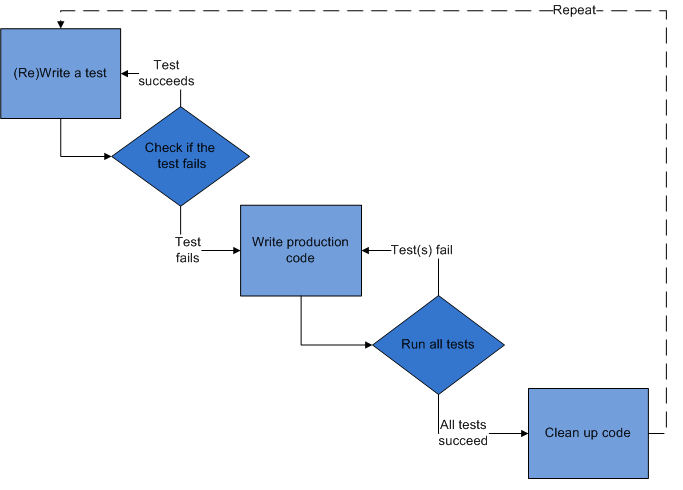
\includegraphics[scale=0.45]{fig/test-driven_development.png}
\end{frame}

\subsection{Characteristics of Test-Driven Development}
\begin{frame}
  \frametitle{Characteristics of Test-Driven Development}\index{test-driven development characteristics}
  \begin{itemize}
    \item \textit{write the test} for a feature \textit{before writing the code}
    \item aids design
      \begin{itemize}
        \item forces systematic thinking about code functionality and interfaces
        \item problem is decomposed into small, modular increments
      \end{itemize}
    \item resulting code is robust and maintainable 
      \begin{itemize}
        \item completely covered by tests
        \item accurate
        \item low coupling, minimal side effects, high cohesion
        \item well-factored, easier to modify
      \end{itemize}
    \item tests are a form of documentation
  \end{itemize}
\end{frame}

\section{Literate Programming}
\begin{frame}
  \frametitle{Literate Programming}
  \begin{itemize}
    \item reverse code/documentation weighting and development cycles
      \begin{itemize}
        \item a lot of code with scant ``comment delimited'' plain text documentation versus
        \item thorough, well-organized, and content-rich documentation with modular and efficient code
      \end{itemize}
    \item high-level language code and associated documentation come from the same set of source files
    \item mathematics and graphics included in documentation
  \end{itemize}
\end{frame}

\subsection{Literate Program Requirements}
\begin{frame}
  \frametitle{Literate Program Requirements\cite{childs}}\index{literate program requirements}
  \begin{enumerate}
    \item code and documentation in same source
    \item documentation and associated code adjacent 
    \item subdivided in a logical way
    \item logical presentation versus conforming to syntactic constraints
    \item includes open issues, rationales, \etc 
    \item description of the problem and solution
      (all the math and graphics necessary)
    \item automatic cross references, indices, and different fonts for text, keywords, 
      variable names, and literals 
    \item written in small chunks including documentation, definitions, and code
  \end{enumerate}
\end{frame}

\subsection{A Quasi-Literate Programming Example}
\begin{frame}[fragile]
  \frametitle{A Quasi-Literate Programming Example}
  We want to integrate the function $f(x) = (2 x-0.5)^3+(1.5 x-1)^2-x+1$ for $x$ in $[0.1,0.8]$
  \begin{columns}[onlytextwidth]
    \begin{column}{0.3\textwidth}
      using the right rectangle numerical integration method. This method is illustrated in 
      the figure to the right.
    \end{column}
    \begin{column}{0.1\textwidth}
    \end{column}
    \begin{column}{0.6\textwidth}
      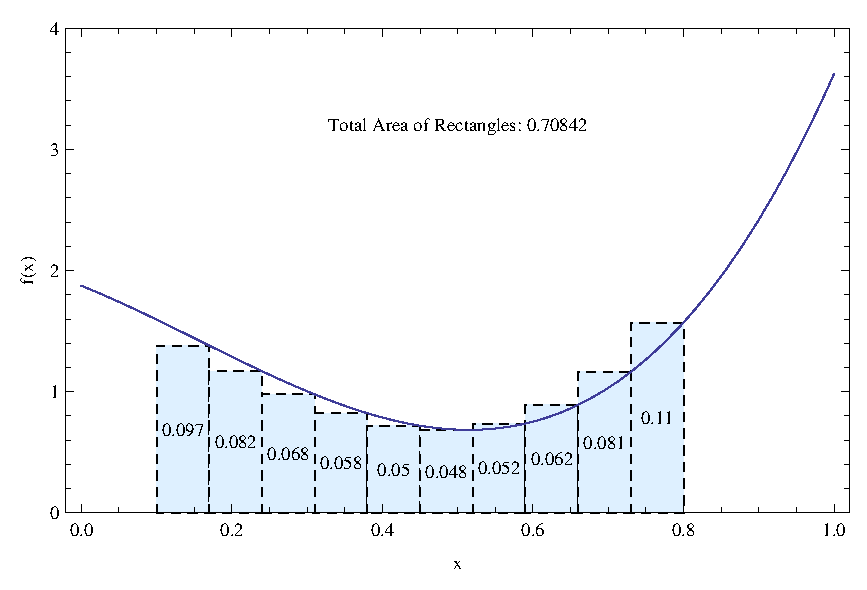
\includegraphics[scale=.45]{../../fig/rightrectangle-10.eps}
    \end{column}
  \end{columns}
  \textit{Helper (testFunctions.chpl)}. Provides the function $f(x) = (2 x-0.5)^3+(1.5 x-1)^2-x+1$.
  \begin{chapel}
proc f(x:real):real {
  return (2 * x - 0.5)**3 + (1.5 * x - 1)**2 - x + 1;
} 
  \end{chapel}
\end{frame}

\subsection{Un-\texttt{tangle} a Literate Program}
\begin{frame}[fragile]
  \frametitle{Un-\texttt{tangle} a Literate Program}\index{tangle}
  \begin{itemize}
    \item typical literate program presented in optimal order for readability 
    \item \texttt{tangle} utility reorganizes code for compiler 
    \item in example below, reference would point to error handling code 
    \item compromise in \seamless 
      \begin{itemize} 
        \item follow TDD but borrow some goodness from literate programming
        \item trade loose coupling and robust testing for code block referencing
      \end{itemize}
  \end{itemize}
  \begin{beamerbox}
    \begin{chapel}
proc readInData(filename:string) {
  var infile = open(filename, iomode.r);
  var reader = infile.reader();

  // 55 lines of error handling code

  readData(reader);
}
    \end{chapel}
  \end{beamerbox}
\end{frame}

\section{\seamless Framework}
\begin{frame}
  \frametitle{\seamless Framework}
  \begin{itemize}
    \item open source tools with a lightweight user interface
      \begin{description}
        \item[user interface:] text editor (\eg vim) + make + \latex + git
        \item[back end:] python + compilers + \latex + cron
      \end{description}
    \item requirements, documentation, specification, source code, and test suite all contained in 
      a \latex document
    \item encourages good software engineering practices: traceability of requirements, robust
      testing, and modular design 
    \item currently supports Chapel (\url{http://chapel.cray.com}), but extensible to other languages
      \index{chapel}
    \item download: \url{http://www.github.com/padamson/seamless}
  \end{itemize}
      \begin{beamerbox}
        \item \texttt{make} // build PDF
        \item \texttt{make sources || tests} // extract source or test code
        \item \texttt{make test} // run tests
      \end{beamerbox}
\end{frame}

\subsection{Documenting Good Requirements}

\begin{frame}
  \index{documenting requirements}
  \frametitle{Documenting Good Requirements}
  \begin{itemize}
    \item failing to write down good requirements is single biggest unnecessary risk
      a developer can take
    \item not understanding requirements diminishes productivity
    \item a thorough requirements specification is crucial for any non-trivial project (more
      than a few days of coding by one programmer)
    \item even trivial projects benefit from an informal specification 
    \item tutorial gives example of scope and functional requirements
      \begin{itemize}
        \item begin with the scope---a brief description of the software package, summarizing the 
          code's high-level capabilities
        \item functional requirements are documented in sufficient detail so that 
          every line of code can be traced back to a requirement
      \end{itemize}
  \end{itemize}
\end{frame}

\begin{frame}
  \frametitle{Documenting Requirements in \seamless}
  \begin{itemize}
    \item requirements are nested in \texttt{description} environments
    \item each labeled item inherits the language of its higher level parents
    \item the most deeply nested items are labeled using the command 
      \texttt{\textbackslash req\{x\}}, where \texttt{x} is the 
      desired number (\eg \texttt{\textbackslash req\{1.1\}}).
  \end{itemize}

  \begin{beamerbox}
    The code shall take inputs \chpl{a} and \chpl{b}
    \begin{description}
      \item and \chpl{c}
        \begin{description}
          \item[\textbf{R1.1}] and compute \chpl{a + b - c}
          \item[\textbf{R1.2}] and compute \chpl{a + b + c}
        \end{description}
      \item[\textbf{R2}] and compute \chpl{a * b}
    \end{description}
  \end{beamerbox}

  \begin{itemize}
    \item \textbf{R1.1:} the code shall take inputs \chpl{a} and \chpl{b} and \chpl{c}
      and compute \chpl{a + b - c}
    \item \textbf{R2:} the code shall take inputs \chpl{a} and \chpl{b} and compute \chpl{a * b}
    \item to reference a requirement, use the command \texttt{\textbackslash ref\{req$@$x\}}, 
      where \texttt{x} is the desired 
      number (\eg \texttt{\textbackslash ref\{req$@$1.1\}}).
  \end{itemize}
\end{frame}

\subsection{Code Development Cycle}
\begin{frame}
  \frametitle{\seamless Code Development Cycle}\index{code development cycle}
  Once requirements are documented, the code development cycle follows:
  \begin{enumerate}
    \item Document a small part of the problem and its solution 
      \begin{enumerate}
        \item Include all aids at your disposal (\eg math, graphics) 
        \item Include references to requirements
      \end{enumerate}
    \item Create a test (or tests, if appropriate) 
      \begin{enumerate}
        \item Keep the tests short
        \item Each test covers only one thing 
        \item The test should run automatically
        \item Make sure the test fails
      \end{enumerate}
    \item Create the code
      \begin{enumerate}
        \item Document and label the code specification, referencing requirements as appropriate
        \item Write the simplest code possible to pass the test
        \item After the test passes, refactor to improve the code
        \item Run the tests again to ensure they still pass
        \item Refactor and retest some more
        \item Update the code specification if necessary
      \end{enumerate}
  \end{enumerate}
\end{frame}

\subsection{Characteristics of Resulting Code}
\begin{frame}
  \frametitle{Characteristics of Resulting Code}
  \begin{itemize}
    \item development cycle repeated until all requirements are met
    \item verify by checking the requirement traceability matrix
    \item process will help to ensure your code has the following characteristics:
      \begin{itemize}
        \item completely documented
        \item simple
        \item readable
        \item completely covered by tests
        \item robust
        \item accurate
        \item maintainable
        \item reusable
      \end{itemize}
  \end{itemize}
\end{frame}

\section{Tutorial}
\subsection{Structure}
\begin{frame}
  \frametitle{Tutorial Structure}
  The files in the provided tutorial can be adapted for your specific application:
  \begin{description}
    \item[\bf Makefile] supports pdflatex and latex to compile the LaTeX package into a
      PDF; also has targets to extract code and run the tests 
    \item[\bf seamless.cls] provides the \seamless document class (a modification of the ``book'' class)
    \item[\bf seamless.sty] provides a few \latex environments and commands 
    \item[\bf Numerical\_Integration.tex] the main \latex document with includes for the remaining LaTeX files 
    \item[\bf chapel\_listing.tex] used with the \latex \texttt{listings} package to properly format Chapel code
    \item[\bf references.bib] contains bibliography entries for use by bibtex
  \end{description}
\end{frame}


\subsection{Notation}
\begin{frame}
  \frametitle{Tutorial Notation}\index{tutorial notation}
    Various environments are defined to highlight different types of notes within color-coded text boxes 
      (\eg \texttt{\textbackslash begin\{TODO\}}
      and \texttt{\textbackslash end\{TODO\}}):

  \begin{TODO}\index{TODO}
    Things that need to be done for the current version of the software. Inserted with \texttt{TODO}
    environment.
  \end{TODO}

  \begin{note-beamer}\index{note}
    Something of note that does not fit into any other category. Inserted with \texttt{note} environment.
  \end{note-beamer}

  \begin{rationale}\index{rationale}
    An explanation for a particular design choice. Inserted with \texttt{rationale} environment.
  \end{rationale}
\end{frame}

\begin{frame}
  \frametitle{Tutorial Notation (continued)}

  \begin{openissue}\index{open issue}\index{open issue}
    Issue that we do not know how to handle. Inserted with \texttt{openissue} environment.
  \end{openissue}

  \begin{future}\index{future}\index{future}
    Issue or feature that we have a story about, but which is not yet
    fully-designed or implemented. Inserted with \texttt{future} environment.
  \end{future}
  In addition, the tutorial contains an additional type of text box to explain background 
  information about the \seamless framework:
  \begin{seamlessnote}\index{seamless note}
    Example text box used to provide background on the \seamless approach in context of the tutorial. 
    Inserted with \texttt{seamlessnote} environment.
  \end{seamlessnote}
\end{frame}

\begin{frame}
  \frametitle{Index}
  \printindex
  %\documentclass{beamer}
\usepackage{beamerthemesplit}
\usetheme{Madrid}
\usecolortheme{seagull}
\usepackage{makeidx}
\usepackage{seamless-beamer}
\usepackage{listings}
\lstdefinelanguage{chapel}
  {
    morekeywords={
      align, atomic,
      begin, bool, break, by,
      class, cobegin, coforall, complex, config, const, continue,
      delete, dmapped, do, domain,
      else, enum, extern, export,
      false, for, forall,
      if, imag, in, index, inline, inout, int, iter,
      label, lambda, let, local, locale,
      module,
      new, nil, noinit,
      on, opaque, otherwise, out,
      param, proc,
      range, real, record, reduce, ref, return,
      scan, select, serial, single, sparse, string, subdomain, sync,
      then, true, type,
      uint, union, use,
      var,
      when, where, while, with,
      yield,
      zip
    },
    sensitive=false,
    mathescape=true,
    morecomment=[l]{//},
    morecomment=[s]{/*}{*/},
    morestring=[b]",
}

\lstset{
    basicstyle=\footnotesize\ttfamily,
    keywordstyle=\bfseries,
    commentstyle=\em,
    showstringspaces=false,
    flexiblecolumns=false,
    numbers=left,
    numbersep=5pt,
    numberstyle=\tiny,
    numberblanklines=false,
    stepnumber=0,
    escapeinside={(*}{*)},
    language=chapel,
  }

%\newcommand{\chpl}[1]{\lstinline[language=chapel,basicstyle=\ttfamily,keywordstyle=\bfseries]!#1!}
\newcommand{\chpl}[1]{\lstinline[language=chapel,basicstyle=\small\ttfamily,keywordstyle=]!#1!}
\newcommand{\varname}[1]{\emph{#1}}
\newcommand{\typename}[1]{\emph{#1}}
\newcommand{\fnname}[1]{\chpl{#1}}

\lstnewenvironment{chapel}{\lstset{language=chapel,xleftmargin=2pc,stepnumber=0}}{}
\lstnewenvironment{invisible}{\lstset{language=chapel,xleftmargin=2pc,stepnumber=0,keywordstyle=\bfseries\color{white},basicstyle=\small\ttfamily\color{white}}}{}
\lstnewenvironment{chapel0}{\lstset{language=chapel,stepnumber=0}}{}

\lstnewenvironment{numberedchapel}{\lstset{language=chapel,xleftmargin=15pt,stepnumber=1}}{}

\lstnewenvironment{chapelcode}{\lstset{language=chapel,stepnumber=1}}{}

% Uses the same listing style as the {chapel} environment, but keyword
% formatting is turned off.  The argument is ignored in LaTeX
% but used to name the .good file during test extraction.
% The argument must be supplied but may be empty.
% If empty it defaults to null, which signals the test extractor to 
% autogenerate the .good file name as ``<test_name>.good''.
\lstnewenvironment{chapelprintoutput}[1]
  {\lstset{language=chapel,xleftmargin=2pc,stepnumber=0,keywordstyle=}}{}

\lstnewenvironment{commandline}{\lstset{keywordstyle=,xleftmargin=2pc}}{}

\lstnewenvironment{protohead}{\lstset{language=chapel,xleftmargin=0pc,belowskip=-10pt,stepnumber=0}}{}

\newenvironment{protobody}{\begin{description}\item[\quad\quad] }{\end{description}}

\renewcommand{\ttdefault}{pcr}
\mode<presentation>
\makeindex
\newenvironment{theindex}
{\let\item\par
  %definitions for subitem etc
}{}
\newcommand\indexspace{}

% some custom latex convenience commands
\usepackage{xspace}
\newcommand*{\eg}{\emph{e.g.}\@\xspace}
\newcommand*{\ie}{\emph{i.e.}\@\xspace}
\newcommand*{\seamless}{\texttt{seamless}\@\xspace}
\newcommand*{\latex}{\LaTeX\@\xspace}

\makeatletter
\newcommand*{\etc}{%
  \@ifnextchar{.}%
  {etc}%
  {etc.\@\xspace}%
}
\makeatother

{ \usetheme{boxes} }
\title[\seamless Introduction]{Code Development with \texttt{seamless}: Introduction}
\author[Adamson]{Paul Adamson \\ \texttt{paul.adamson.01@gmail.com}}
\date{January 29, 2015}

%\AtBeginSection[]
%{
  %\begin{frame}
    %\frametitle{Outline}
    %\tableofcontents[currentsection]
  %\end{frame}
%}

\begin{document}
\begin{frame}
  \titlepage
\end{frame}

\begin{frame}
  \frametitle{Outline}
  \tableofcontents
\end{frame}

\section{Motivation for \texttt{seamless}}
\begin{frame}
  \frametitle{Motivation for \seamless}
  \begin{itemize}
    \item a lot of legacy code will be rewritten over the next couple of decades
    \item many incentives to producing reusable, maintainable code\cite{petre}
    \item some significant roadblocks 
      \begin{itemize}
        \item we are scientists first, programmers second (or third, fourth...)
        \item high overhead of integrating multiple software engineering tools
        \item we think $cost > benefit$
      \end{itemize}
    \item need a lightweight, easy to use system to implement good software engineering
      practices
    \item targeting small- to moderately-sized software projects
    \item not looking to develop a template for all projects---tool will be extensible \& adaptable
  \end{itemize}
\end{frame}


\section{Test-Driven Development}
\subsection{Typical Test-Driven Development (TDD) Process}
\begin{frame}
  \frametitle{Typical Test-Driven Development (TDD) Process\cite{tdd-wikipedia}}
\index{test-driven development process}
  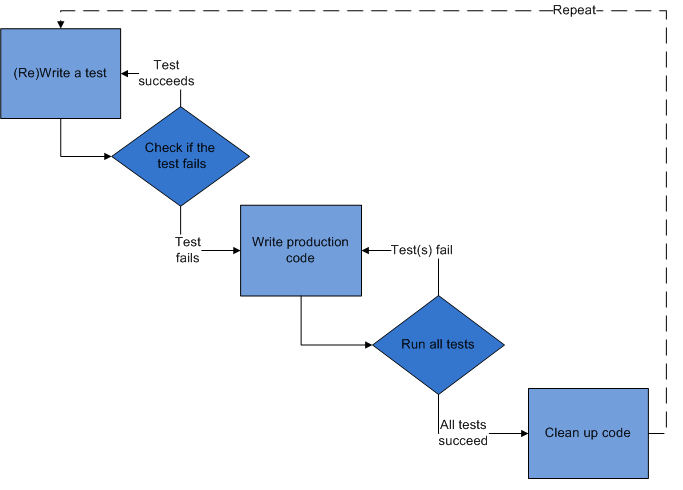
\includegraphics[scale=0.45]{fig/test-driven_development.png}
\end{frame}

\subsection{Characteristics of Test-Driven Development}
\begin{frame}
  \frametitle{Characteristics of Test-Driven Development}\index{test-driven development characteristics}
  \begin{itemize}
    \item \textit{write the test} for a feature \textit{before writing the code}
    \item aids design
      \begin{itemize}
        \item forces systematic thinking about code functionality and interfaces
        \item problem is decomposed into small, modular increments
      \end{itemize}
    \item resulting code is robust and maintainable 
      \begin{itemize}
        \item completely covered by tests
        \item accurate
        \item low coupling, minimal side effects, high cohesion
        \item well-factored, easier to modify
      \end{itemize}
    \item tests are a form of documentation
  \end{itemize}
\end{frame}

\section{Literate Programming}
\begin{frame}
  \frametitle{Literate Programming}
  \begin{itemize}
    \item reverse code/documentation weighting and development cycles
      \begin{itemize}
        \item a lot of code with scant ``comment delimited'' plain text documentation versus
        \item thorough, well-organized, and content-rich documentation with modular and efficient code
      \end{itemize}
    \item high-level language code and associated documentation come from the same set of source files
    \item mathematics and graphics included in documentation
  \end{itemize}
\end{frame}

\subsection{Literate Program Requirements}
\begin{frame}
  \frametitle{Literate Program Requirements\cite{childs}}\index{literate program requirements}
  \begin{enumerate}
    \item code and documentation in same source
    \item documentation and associated code adjacent 
    \item subdivided in a logical way
    \item logical presentation versus conforming to syntactic constraints
    \item includes open issues, rationales, \etc 
    \item description of the problem and solution
      (all the math and graphics necessary)
    \item automatic cross references, indices, and different fonts for text, keywords, 
      variable names, and literals 
    \item written in small chunks including documentation, definitions, and code
  \end{enumerate}
\end{frame}

\subsection{A Quasi-Literate Programming Example}
\begin{frame}[fragile]
  \frametitle{A Quasi-Literate Programming Example}
  We want to integrate the function $f(x) = (2 x-0.5)^3+(1.5 x-1)^2-x+1$ for $x$ in $[0.1,0.8]$
  \begin{columns}[onlytextwidth]
    \begin{column}{0.3\textwidth}
      using the right rectangle numerical integration method. This method is illustrated in 
      the figure to the right.
    \end{column}
    \begin{column}{0.1\textwidth}
    \end{column}
    \begin{column}{0.6\textwidth}
      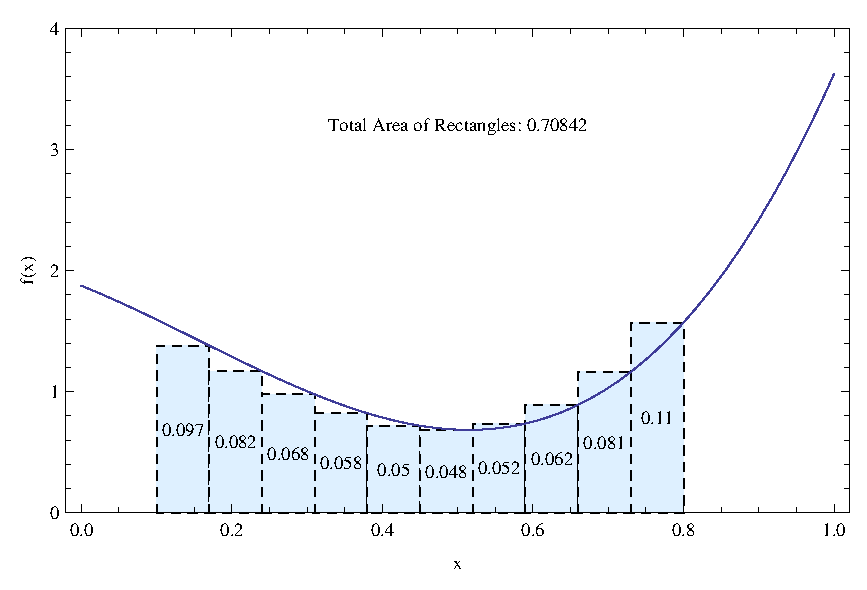
\includegraphics[scale=.45]{../../fig/rightrectangle-10.eps}
    \end{column}
  \end{columns}
  \textit{Helper (testFunctions.chpl)}. Provides the function $f(x) = (2 x-0.5)^3+(1.5 x-1)^2-x+1$.
  \begin{chapel}
proc f(x:real):real {
  return (2 * x - 0.5)**3 + (1.5 * x - 1)**2 - x + 1;
} 
  \end{chapel}
\end{frame}

\subsection{Un-\texttt{tangle} a Literate Program}
\begin{frame}[fragile]
  \frametitle{Un-\texttt{tangle} a Literate Program}\index{tangle}
  \begin{itemize}
    \item typical literate program presented in optimal order for readability 
    \item \texttt{tangle} utility reorganizes code for compiler 
    \item in example below, reference would point to error handling code 
    \item compromise in \seamless 
      \begin{itemize} 
        \item follow TDD but borrow some goodness from literate programming
        \item trade loose coupling and robust testing for code block referencing
      \end{itemize}
  \end{itemize}
  \begin{beamerbox}
    \begin{chapel}
proc readInData(filename:string) {
  var infile = open(filename, iomode.r);
  var reader = infile.reader();

  // 55 lines of error handling code

  readData(reader);
}
    \end{chapel}
  \end{beamerbox}
\end{frame}

\section{\seamless Framework}
\begin{frame}
  \frametitle{\seamless Framework}
  \begin{itemize}
    \item open source tools with a lightweight user interface
      \begin{description}
        \item[user interface:] text editor (\eg vim) + make + \latex + git
        \item[back end:] python + compilers + \latex + cron
      \end{description}
    \item requirements, documentation, specification, source code, and test suite all contained in 
      a \latex document
    \item encourages good software engineering practices: traceability of requirements, robust
      testing, and modular design 
    \item currently supports Chapel (\url{http://chapel.cray.com}), but extensible to other languages
      \index{chapel}
    \item download: \url{http://www.github.com/padamson/seamless}
  \end{itemize}
      \begin{beamerbox}
        \item \texttt{make} // build PDF
        \item \texttt{make sources || tests} // extract source or test code
        \item \texttt{make test} // run tests
      \end{beamerbox}
\end{frame}

\subsection{Documenting Good Requirements}

\begin{frame}
  \index{documenting requirements}
  \frametitle{Documenting Good Requirements}
  \begin{itemize}
    \item failing to write down good requirements is single biggest unnecessary risk
      a developer can take
    \item not understanding requirements diminishes productivity
    \item a thorough requirements specification is crucial for any non-trivial project (more
      than a few days of coding by one programmer)
    \item even trivial projects benefit from an informal specification 
    \item tutorial gives example of scope and functional requirements
      \begin{itemize}
        \item begin with the scope---a brief description of the software package, summarizing the 
          code's high-level capabilities
        \item functional requirements are documented in sufficient detail so that 
          every line of code can be traced back to a requirement
      \end{itemize}
  \end{itemize}
\end{frame}

\begin{frame}
  \frametitle{Documenting Requirements in \seamless}
  \begin{itemize}
    \item requirements are nested in \texttt{description} environments
    \item each labeled item inherits the language of its higher level parents
    \item the most deeply nested items are labeled using the command 
      \texttt{\textbackslash req\{x\}}, where \texttt{x} is the 
      desired number (\eg \texttt{\textbackslash req\{1.1\}}).
  \end{itemize}

  \begin{beamerbox}
    The code shall take inputs \chpl{a} and \chpl{b}
    \begin{description}
      \item and \chpl{c}
        \begin{description}
          \item[\textbf{R1.1}] and compute \chpl{a + b - c}
          \item[\textbf{R1.2}] and compute \chpl{a + b + c}
        \end{description}
      \item[\textbf{R2}] and compute \chpl{a * b}
    \end{description}
  \end{beamerbox}

  \begin{itemize}
    \item \textbf{R1.1:} the code shall take inputs \chpl{a} and \chpl{b} and \chpl{c}
      and compute \chpl{a + b - c}
    \item \textbf{R2:} the code shall take inputs \chpl{a} and \chpl{b} and compute \chpl{a * b}
    \item to reference a requirement, use the command \texttt{\textbackslash ref\{req$@$x\}}, 
      where \texttt{x} is the desired 
      number (\eg \texttt{\textbackslash ref\{req$@$1.1\}}).
  \end{itemize}
\end{frame}

\subsection{Code Development Cycle}
\begin{frame}
  \frametitle{\seamless Code Development Cycle}\index{code development cycle}
  Once requirements are documented, the code development cycle follows:
  \begin{enumerate}
    \item Document a small part of the problem and its solution 
      \begin{enumerate}
        \item Include all aids at your disposal (\eg math, graphics) 
        \item Include references to requirements
      \end{enumerate}
    \item Create a test (or tests, if appropriate) 
      \begin{enumerate}
        \item Keep the tests short
        \item Each test covers only one thing 
        \item The test should run automatically
        \item Make sure the test fails
      \end{enumerate}
    \item Create the code
      \begin{enumerate}
        \item Document and label the code specification, referencing requirements as appropriate
        \item Write the simplest code possible to pass the test
        \item After the test passes, refactor to improve the code
        \item Run the tests again to ensure they still pass
        \item Refactor and retest some more
        \item Update the code specification if necessary
      \end{enumerate}
  \end{enumerate}
\end{frame}

\subsection{Characteristics of Resulting Code}
\begin{frame}
  \frametitle{Characteristics of Resulting Code}
  \begin{itemize}
    \item development cycle repeated until all requirements are met
    \item verify by checking the requirement traceability matrix
    \item process will help to ensure your code has the following characteristics:
      \begin{itemize}
        \item completely documented
        \item simple
        \item readable
        \item completely covered by tests
        \item robust
        \item accurate
        \item maintainable
        \item reusable
      \end{itemize}
  \end{itemize}
\end{frame}

\section{Tutorial}
\subsection{Structure}
\begin{frame}
  \frametitle{Tutorial Structure}
  The files in the provided tutorial can be adapted for your specific application:
  \begin{description}
    \item[\bf Makefile] supports pdflatex and latex to compile the LaTeX package into a
      PDF; also has targets to extract code and run the tests 
    \item[\bf seamless.cls] provides the \seamless document class (a modification of the ``book'' class)
    \item[\bf seamless.sty] provides a few \latex environments and commands 
    \item[\bf Numerical\_Integration.tex] the main \latex document with includes for the remaining LaTeX files 
    \item[\bf chapel\_listing.tex] used with the \latex \texttt{listings} package to properly format Chapel code
    \item[\bf references.bib] contains bibliography entries for use by bibtex
  \end{description}
\end{frame}


\subsection{Notation}
\begin{frame}
  \frametitle{Tutorial Notation}\index{tutorial notation}
    Various environments are defined to highlight different types of notes within color-coded text boxes 
      (\eg \texttt{\textbackslash begin\{TODO\}}
      and \texttt{\textbackslash end\{TODO\}}):

  \begin{TODO}\index{TODO}
    Things that need to be done for the current version of the software. Inserted with \texttt{TODO}
    environment.
  \end{TODO}

  \begin{note-beamer}\index{note}
    Something of note that does not fit into any other category. Inserted with \texttt{note} environment.
  \end{note-beamer}

  \begin{rationale}\index{rationale}
    An explanation for a particular design choice. Inserted with \texttt{rationale} environment.
  \end{rationale}
\end{frame}

\begin{frame}
  \frametitle{Tutorial Notation (continued)}

  \begin{openissue}\index{open issue}\index{open issue}
    Issue that we do not know how to handle. Inserted with \texttt{openissue} environment.
  \end{openissue}

  \begin{future}\index{future}\index{future}
    Issue or feature that we have a story about, but which is not yet
    fully-designed or implemented. Inserted with \texttt{future} environment.
  \end{future}
  In addition, the tutorial contains an additional type of text box to explain background 
  information about the \seamless framework:
  \begin{seamlessnote}\index{seamless note}
    Example text box used to provide background on the \seamless approach in context of the tutorial. 
    Inserted with \texttt{seamlessnote} environment.
  \end{seamlessnote}
\end{frame}

\begin{frame}
  \frametitle{Index}
  \printindex
  %\documentclass{beamer}
\usepackage{beamerthemesplit}
\usetheme{Madrid}
\usecolortheme{seagull}
\usepackage{makeidx}
\usepackage{seamless-beamer}
\usepackage{listings}
\input{../../chapel_listing}
\renewcommand{\ttdefault}{pcr}
\mode<presentation>
\makeindex
\newenvironment{theindex}
{\let\item\par
  %definitions for subitem etc
}{}
\newcommand\indexspace{}

% some custom latex convenience commands
\usepackage{xspace}
\newcommand*{\eg}{\emph{e.g.}\@\xspace}
\newcommand*{\ie}{\emph{i.e.}\@\xspace}
\newcommand*{\seamless}{\texttt{seamless}\@\xspace}
\newcommand*{\latex}{\LaTeX\@\xspace}

\makeatletter
\newcommand*{\etc}{%
  \@ifnextchar{.}%
  {etc}%
  {etc.\@\xspace}%
}
\makeatother

{ \usetheme{boxes} }
\title[\seamless Introduction]{Code Development with \texttt{seamless}: Introduction}
\author[Adamson]{Paul Adamson \\ \texttt{paul.adamson.01@gmail.com}}
\date{January 29, 2015}

%\AtBeginSection[]
%{
  %\begin{frame}
    %\frametitle{Outline}
    %\tableofcontents[currentsection]
  %\end{frame}
%}

\begin{document}
\begin{frame}
  \titlepage
\end{frame}

\begin{frame}
  \frametitle{Outline}
  \tableofcontents
\end{frame}

\section{Motivation for \texttt{seamless}}
\begin{frame}
  \frametitle{Motivation for \seamless}
  \begin{itemize}
    \item a lot of legacy code will be rewritten over the next couple of decades
    \item many incentives to producing reusable, maintainable code\cite{petre}
    \item some significant roadblocks 
      \begin{itemize}
        \item we are scientists first, programmers second (or third, fourth...)
        \item high overhead of integrating multiple software engineering tools
        \item we think $cost > benefit$
      \end{itemize}
    \item need a lightweight, easy to use system to implement good software engineering
      practices
    \item targeting small- to moderately-sized software projects
    \item not looking to develop a template for all projects---tool will be extensible \& adaptable
  \end{itemize}
\end{frame}


\section{Test-Driven Development}
\subsection{Typical Test-Driven Development (TDD) Process}
\begin{frame}
  \frametitle{Typical Test-Driven Development (TDD) Process\cite{tdd-wikipedia}}
\index{test-driven development process}
  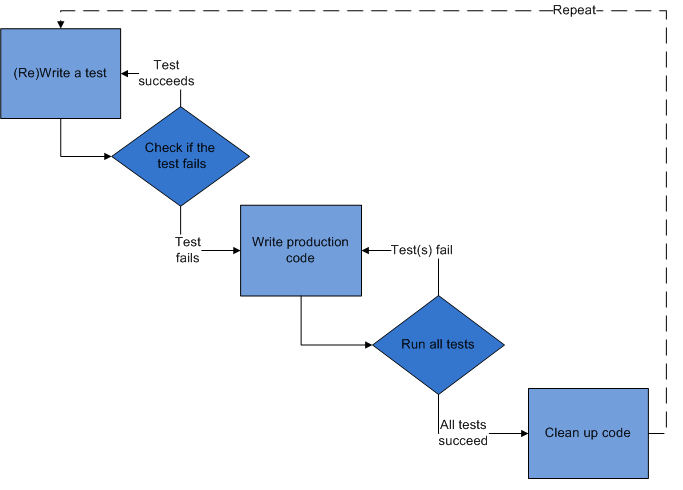
\includegraphics[scale=0.45]{fig/test-driven_development.png}
\end{frame}

\subsection{Characteristics of Test-Driven Development}
\begin{frame}
  \frametitle{Characteristics of Test-Driven Development}\index{test-driven development characteristics}
  \begin{itemize}
    \item \textit{write the test} for a feature \textit{before writing the code}
    \item aids design
      \begin{itemize}
        \item forces systematic thinking about code functionality and interfaces
        \item problem is decomposed into small, modular increments
      \end{itemize}
    \item resulting code is robust and maintainable 
      \begin{itemize}
        \item completely covered by tests
        \item accurate
        \item low coupling, minimal side effects, high cohesion
        \item well-factored, easier to modify
      \end{itemize}
    \item tests are a form of documentation
  \end{itemize}
\end{frame}

\section{Literate Programming}
\begin{frame}
  \frametitle{Literate Programming}
  \begin{itemize}
    \item reverse code/documentation weighting and development cycles
      \begin{itemize}
        \item a lot of code with scant ``comment delimited'' plain text documentation versus
        \item thorough, well-organized, and content-rich documentation with modular and efficient code
      \end{itemize}
    \item high-level language code and associated documentation come from the same set of source files
    \item mathematics and graphics included in documentation
  \end{itemize}
\end{frame}

\subsection{Literate Program Requirements}
\begin{frame}
  \frametitle{Literate Program Requirements\cite{childs}}\index{literate program requirements}
  \begin{enumerate}
    \item code and documentation in same source
    \item documentation and associated code adjacent 
    \item subdivided in a logical way
    \item logical presentation versus conforming to syntactic constraints
    \item includes open issues, rationales, \etc 
    \item description of the problem and solution
      (all the math and graphics necessary)
    \item automatic cross references, indices, and different fonts for text, keywords, 
      variable names, and literals 
    \item written in small chunks including documentation, definitions, and code
  \end{enumerate}
\end{frame}

\subsection{A Quasi-Literate Programming Example}
\begin{frame}[fragile]
  \frametitle{A Quasi-Literate Programming Example}
  We want to integrate the function $f(x) = (2 x-0.5)^3+(1.5 x-1)^2-x+1$ for $x$ in $[0.1,0.8]$
  \begin{columns}[onlytextwidth]
    \begin{column}{0.3\textwidth}
      using the right rectangle numerical integration method. This method is illustrated in 
      the figure to the right.
    \end{column}
    \begin{column}{0.1\textwidth}
    \end{column}
    \begin{column}{0.6\textwidth}
      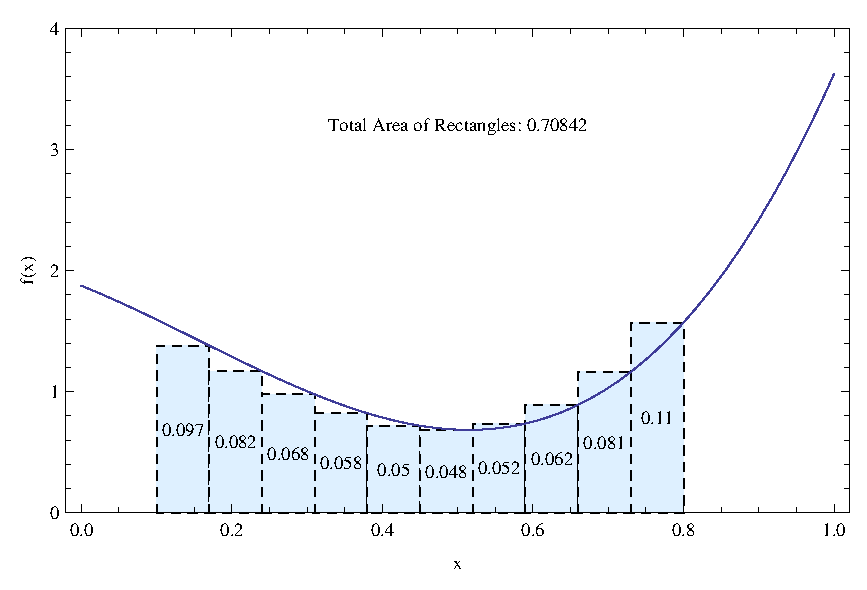
\includegraphics[scale=.45]{../../fig/rightrectangle-10.eps}
    \end{column}
  \end{columns}
  \textit{Helper (testFunctions.chpl)}. Provides the function $f(x) = (2 x-0.5)^3+(1.5 x-1)^2-x+1$.
  \begin{chapel}
proc f(x:real):real {
  return (2 * x - 0.5)**3 + (1.5 * x - 1)**2 - x + 1;
} 
  \end{chapel}
\end{frame}

\subsection{Un-\texttt{tangle} a Literate Program}
\begin{frame}[fragile]
  \frametitle{Un-\texttt{tangle} a Literate Program}\index{tangle}
  \begin{itemize}
    \item typical literate program presented in optimal order for readability 
    \item \texttt{tangle} utility reorganizes code for compiler 
    \item in example below, reference would point to error handling code 
    \item compromise in \seamless 
      \begin{itemize} 
        \item follow TDD but borrow some goodness from literate programming
        \item trade loose coupling and robust testing for code block referencing
      \end{itemize}
  \end{itemize}
  \begin{beamerbox}
    \begin{chapel}
proc readInData(filename:string) {
  var infile = open(filename, iomode.r);
  var reader = infile.reader();

  // 55 lines of error handling code

  readData(reader);
}
    \end{chapel}
  \end{beamerbox}
\end{frame}

\section{\seamless Framework}
\begin{frame}
  \frametitle{\seamless Framework}
  \begin{itemize}
    \item open source tools with a lightweight user interface
      \begin{description}
        \item[user interface:] text editor (\eg vim) + make + \latex + git
        \item[back end:] python + compilers + \latex + cron
      \end{description}
    \item requirements, documentation, specification, source code, and test suite all contained in 
      a \latex document
    \item encourages good software engineering practices: traceability of requirements, robust
      testing, and modular design 
    \item currently supports Chapel (\url{http://chapel.cray.com}), but extensible to other languages
      \index{chapel}
    \item download: \url{http://www.github.com/padamson/seamless}
  \end{itemize}
      \begin{beamerbox}
        \item \texttt{make} // build PDF
        \item \texttt{make sources || tests} // extract source or test code
        \item \texttt{make test} // run tests
      \end{beamerbox}
\end{frame}

\subsection{Documenting Good Requirements}

\begin{frame}
  \index{documenting requirements}
  \frametitle{Documenting Good Requirements}
  \begin{itemize}
    \item failing to write down good requirements is single biggest unnecessary risk
      a developer can take
    \item not understanding requirements diminishes productivity
    \item a thorough requirements specification is crucial for any non-trivial project (more
      than a few days of coding by one programmer)
    \item even trivial projects benefit from an informal specification 
    \item tutorial gives example of scope and functional requirements
      \begin{itemize}
        \item begin with the scope---a brief description of the software package, summarizing the 
          code's high-level capabilities
        \item functional requirements are documented in sufficient detail so that 
          every line of code can be traced back to a requirement
      \end{itemize}
  \end{itemize}
\end{frame}

\begin{frame}
  \frametitle{Documenting Requirements in \seamless}
  \begin{itemize}
    \item requirements are nested in \texttt{description} environments
    \item each labeled item inherits the language of its higher level parents
    \item the most deeply nested items are labeled using the command 
      \texttt{\textbackslash req\{x\}}, where \texttt{x} is the 
      desired number (\eg \texttt{\textbackslash req\{1.1\}}).
  \end{itemize}

  \begin{beamerbox}
    The code shall take inputs \chpl{a} and \chpl{b}
    \begin{description}
      \item and \chpl{c}
        \begin{description}
          \item[\textbf{R1.1}] and compute \chpl{a + b - c}
          \item[\textbf{R1.2}] and compute \chpl{a + b + c}
        \end{description}
      \item[\textbf{R2}] and compute \chpl{a * b}
    \end{description}
  \end{beamerbox}

  \begin{itemize}
    \item \textbf{R1.1:} the code shall take inputs \chpl{a} and \chpl{b} and \chpl{c}
      and compute \chpl{a + b - c}
    \item \textbf{R2:} the code shall take inputs \chpl{a} and \chpl{b} and compute \chpl{a * b}
    \item to reference a requirement, use the command \texttt{\textbackslash ref\{req$@$x\}}, 
      where \texttt{x} is the desired 
      number (\eg \texttt{\textbackslash ref\{req$@$1.1\}}).
  \end{itemize}
\end{frame}

\subsection{Code Development Cycle}
\begin{frame}
  \frametitle{\seamless Code Development Cycle}\index{code development cycle}
  Once requirements are documented, the code development cycle follows:
  \begin{enumerate}
    \item Document a small part of the problem and its solution 
      \begin{enumerate}
        \item Include all aids at your disposal (\eg math, graphics) 
        \item Include references to requirements
      \end{enumerate}
    \item Create a test (or tests, if appropriate) 
      \begin{enumerate}
        \item Keep the tests short
        \item Each test covers only one thing 
        \item The test should run automatically
        \item Make sure the test fails
      \end{enumerate}
    \item Create the code
      \begin{enumerate}
        \item Document and label the code specification, referencing requirements as appropriate
        \item Write the simplest code possible to pass the test
        \item After the test passes, refactor to improve the code
        \item Run the tests again to ensure they still pass
        \item Refactor and retest some more
        \item Update the code specification if necessary
      \end{enumerate}
  \end{enumerate}
\end{frame}

\subsection{Characteristics of Resulting Code}
\begin{frame}
  \frametitle{Characteristics of Resulting Code}
  \begin{itemize}
    \item development cycle repeated until all requirements are met
    \item verify by checking the requirement traceability matrix
    \item process will help to ensure your code has the following characteristics:
      \begin{itemize}
        \item completely documented
        \item simple
        \item readable
        \item completely covered by tests
        \item robust
        \item accurate
        \item maintainable
        \item reusable
      \end{itemize}
  \end{itemize}
\end{frame}

\section{Tutorial}
\subsection{Structure}
\begin{frame}
  \frametitle{Tutorial Structure}
  The files in the provided tutorial can be adapted for your specific application:
  \begin{description}
    \item[\bf Makefile] supports pdflatex and latex to compile the LaTeX package into a
      PDF; also has targets to extract code and run the tests 
    \item[\bf seamless.cls] provides the \seamless document class (a modification of the ``book'' class)
    \item[\bf seamless.sty] provides a few \latex environments and commands 
    \item[\bf Numerical\_Integration.tex] the main \latex document with includes for the remaining LaTeX files 
    \item[\bf chapel\_listing.tex] used with the \latex \texttt{listings} package to properly format Chapel code
    \item[\bf references.bib] contains bibliography entries for use by bibtex
  \end{description}
\end{frame}


\subsection{Notation}
\begin{frame}
  \frametitle{Tutorial Notation}\index{tutorial notation}
    Various environments are defined to highlight different types of notes within color-coded text boxes 
      (\eg \texttt{\textbackslash begin\{TODO\}}
      and \texttt{\textbackslash end\{TODO\}}):

  \begin{TODO}\index{TODO}
    Things that need to be done for the current version of the software. Inserted with \texttt{TODO}
    environment.
  \end{TODO}

  \begin{note-beamer}\index{note}
    Something of note that does not fit into any other category. Inserted with \texttt{note} environment.
  \end{note-beamer}

  \begin{rationale}\index{rationale}
    An explanation for a particular design choice. Inserted with \texttt{rationale} environment.
  \end{rationale}
\end{frame}

\begin{frame}
  \frametitle{Tutorial Notation (continued)}

  \begin{openissue}\index{open issue}\index{open issue}
    Issue that we do not know how to handle. Inserted with \texttt{openissue} environment.
  \end{openissue}

  \begin{future}\index{future}\index{future}
    Issue or feature that we have a story about, but which is not yet
    fully-designed or implemented. Inserted with \texttt{future} environment.
  \end{future}
  In addition, the tutorial contains an additional type of text box to explain background 
  information about the \seamless framework:
  \begin{seamlessnote}\index{seamless note}
    Example text box used to provide background on the \seamless approach in context of the tutorial. 
    Inserted with \texttt{seamlessnote} environment.
  \end{seamlessnote}
\end{frame}

\begin{frame}
  \frametitle{Index}
  \printindex
  %\input{seamless-intro.idx}
\end{frame}

\begin{frame}
  \frametitle{References}
  \bibliographystyle{plain}       
  \bibliography{references} 
\end{frame}

\end{document}

\end{frame}

\begin{frame}
  \frametitle{References}
  \bibliographystyle{plain}       
  \bibliography{references} 
\end{frame}

\end{document}

\end{frame}

\begin{frame}
  \frametitle{References}
  \bibliographystyle{plain}       
  \bibliography{references} 
\end{frame}

\end{document}

\end{frame}

\begin{frame}
  \frametitle{References}
  \bibliographystyle{plain}       
  \bibliography{references} 
\end{frame}

\end{document}
